\section{Initialization choices}

In this project, two different initializations for the weight and bias are implemented. 
For the TanH layer, the initialization used is the Xavier one. 
Thus the weights are initialized from a random distribution with a mean of $0$ and a variance of $\dfrac{2}{size^{Layer-1}+size^{Layer}}$ and the biases to $0$. 
For the ReLu layer, the initialization used is the He one. 
It is the same initialization as the Xavier one, but with twice the variance. 
Those initializations help to reduce the risk that the gradients vanish or explode.

\begin{figure}[H]
	\begin{subfigure}[h]{0.35\textwidth}
		\begin{center}
			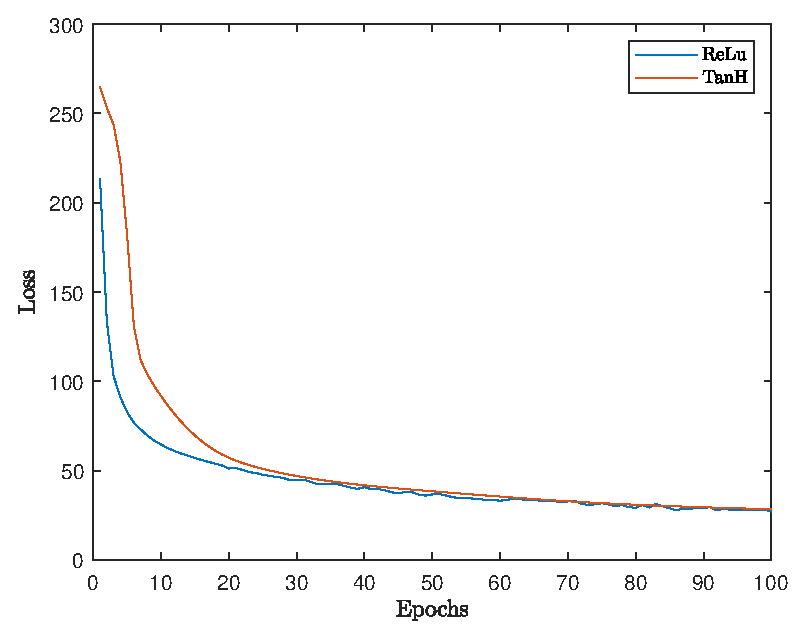
\includegraphics[width=\textwidth]{loss}
		\end{center}
	\end{subfigure}
	\begin{subfigure}[h]{0.35\textwidth}
		\begin{center}
			\includegraphics[width=\textwidth]{accuracy}
		\end{center}
	\end{subfigure}
	\caption{Average of 5 measures of loss and accuracy of a neural network with $2$ inputs and  outputs, and $3$ hidden layers of $25$ neurons each, with the following parameters : $100$ epochs, batch size of $1$, learning rate of $0.02$.}
	\label{img::loss_accuracy}
\end{figure}

On Figure~\ref{img::loss_accuracy}, we can see the result of two neural networks with $2$ inputs, $2$ outputs and $3$ hidden layers of $25$ neurons each. 
The blue one is with ReLu layers and the red on is with TanH layers. 
We can see that the loss converges for the two types of layer. 
With the chosen parameters, we can see that TanH has a better accuracy but is slower to converge than the ReLu layer. 
The initialization was also tested with a variance of $1$, but with this parameter the loss diverges.